%!TEX encoding = UTF8
%!TEX root =notes.tex
\chapter{Probabilités}

Le but de ce chapitre est d'étudier la notion de loi de probabilité sur un ensemble d'issues.
Une loi de probabilité est une hypothèse de départ choisie pour modéliser la réalité.
Celle-ci ne se démontre pas et peut résulter soit d'hypothèses théoriques, soit à partir de fréquences observées après un grand nombre d'expériences.
Cette deuxième méthode s'appuie sur le fait que la fréquence d'un événement s'approche de sa probabilité lorsque le nombre d'expériences augmente.
On appelle ce résultat la \og loi des grands nombres \fg.

Les objectifs de ce chapitre sont les suivants, tels que listés dans le bulletin officiel.
	\begin{enumerate}
		\item Ensemble (univers) des issues. Événements. Réunion, intersection, complémentaire.
		\item Loi (distribution) de probabilité. Probabilité d'un événement : somme des probabilités des issues.
		\item Relation $P(A \cup B) + P(A \cap B) = P(A) + P(B)$.
		\item Dénombrement à l'aide de tableaux et d'arbres.
	\end{enumerate}
Les capacités visées sont les suivantes.
	\begin{enumerate}
		\item Utiliser des modèles théoriques de référence en comprenant que les probabilités sont définies a priori.
		\item Construire un modèle à partir de fréquences observées, en distinguant nettement modèle et réalité.
		\item Calculer des probabilités dans des cas simples : expérience aléatoire à deux ou trois épreuves.
	\end{enumerate}

\section{Introduction}

On introduit ici le concept d'univers et d'événement à l'aide d'ensembles finis.

\dfn{Expérience aléatoire}{
	Une expérience aléatoire est une expérience renouvelable dont on connait les résulats possibles sans qu'on puisse savoir avec certitude lequel sera réalisé.
}{}

\dfn{Univers $\Omega$}{
	L'universe $\Omega$ d'une expérience aléatoire est l'\textbf{ensemble} des issues possibles.
}{}

\ex{}{
	On tire deux cartes d'un jeu complet et on considère les couleurs des cartes tirées, sans les ordonner.
	Les $10$ issues possibles constituent l'univers :
		\[
		\Omega = \left\{
		\begin{aligned}
			&( \clubsuit, \clubsuit ), ( \clubsuit, \heartsuit ), ( \clubsuit, \spadesuit ), \\ 
			&( \clubsuit, \diamondsuit ), ( \heartsuit, \heartsuit ), ( \heartsuit, \spadesuit ), \\
			&( \heartsuit, \diamondsuit ), ( \spadesuit, \spadesuit ), ( \spadesuit, \diamondsuit ), ( \diamondsuit, \diamondsuit )
		\end{aligned}
		\right\}
		\]
	Remarquons que si on avait choisi d'ordonner les cartes (en choisir une première puis une deuxième), on aurait plutôt $16$ issues possibles, car dans ce cas $(\clubsuit, \heartsuit) \neq (\heartsuit, \clubsuit)$
}{ex:2-cartes}

\exe{}{
	Donner les univers $\Omega$ des expériences aléatoires suivantes.
	\begin{multicols}{2}
	\begin{enumerate}[label=---]
		\item Un lancer de dé équilibré à six faces.
		\item Un lancer de pièce de monnaie.
		\item Chiffres du loto.
		\item Un lancer de dé pipé (truqué) à six faces.
	\end{enumerate}
	\end{multicols}
}{}

\dfn{Événement}{
	Un \emph{événement} est un sous-ensemble de l'univers.
	On peut le décrire avec un ensemble ou des mots, par abus de notation.
}{}

\ex{}{
	Dans l'expérience aléatoire de l'exemple \ref{ex:2-cartes}, on considère l'événement $E$ suivant.
		\begin{center}
			E : \og au moins une carte de carreau est tirée \fg.
		\end{center}
	Cet événement est associé à l'ensemble $S$ des issues de l'univers $\Omega$ vérifiant $E$.
	C'est-à-dire l'ensemble des paires de couleurs dont au moins une est de carreau.
		\begin{align*}
			S &= \{ c \in \Omega \text{ tels qu'au moins une des cartes du couple $c$ est de carreau} \} \\
			&= \left\{
			\begin{aligned}
			&( \clubsuit, \diamondsuit ), ( \heartsuit, \diamondsuit ), \\
			&( \spadesuit, \diamondsuit ), ( \diamondsuit, \diamondsuit )
			\end{aligned}
			\right\}
		\end{align*}
	Il y a $4$ issues possibles correspondant à cet événement.
}{}

\section{Lois de probabilité}

Lorsqu'on considère une expérience aléatoire, on associe une probabilité à chaque issue possible (c'est-à-dire chaque élément de l'univers).
C'est association est une loi de probabilité qu'on ne démontre jamais : c'est la base de la modélisation du hasard.

\dfn{Loi de probabilité}{
	Soit $\Omega = \{ \omega_1, \omega_2, \omega_3, \dots \}$ un univers fini.
	Une loi de probabilité $P$ est une fonction associant à chaque issue $\omega$ une valeur de $[0;1]$ (sa probabilité d'être réalisée).
	\begin{center}
	\begin{tabular}{|c|c|c|c|} \hline
		Issue		& $\omega_1$ & $\omega_2$ & \hspace{15pt} \dots \hspace{15pt} \\ \hline
		Probabilité	& $P(\omega_1)$ & $P(\omega_2)$ &\hspace{15pt} \dots \hspace{15pt} \\ \hline
	\end{tabular}
	\end{center}
	La loi $P$ s'étend à tout sous-ensemble $E = \{e_1, e_2, \dots \}$ de l'univers $\Omega$ par additivité : la probabilité de l'événement $E$ est la somme de la probabilité de chacun de ses éléments.
			\[ P(E) = P(e_1) + P(e_2) + \dots \]
	En outre, la probabilité de l'univers tout entier est $1$ :
		\[ P(\Omega) = P(\omega_1) + P(\omega_2) + \dots  = 1, \]
	et la probabilité de l'ensemble vide $\emptyset$ est nulle :
		\[ P(\emptyset) = 0. \]
}{}

\nt{
	En écrivant $P(\omega)$, on abuse légèrement d'une notation. Il faudrait plutôt écrire
		\[ P(\{\omega\}), \]
	car la fonction $P$ prend uniquement des sous-ensembles de $\Omega$.
}{}

\thm{Inclusion-exclusion}{
	Soient $A, B \subseteq \Omega$ deux événements.
	Alors
		\[ P(A \cup B) = P(A) + P(B) - P(A\cap B). \]
}{thm:incl-excl}

\pf{Preuve du théorème \ref{thm:incl-excl}}{
	On considère les diagrammes de Venn suivants.
	\begin{center}
	\begin{tikzpicture}[fill=gray, scale=1]
		% left hand
		\scope
		\draw[pattern=north west lines, pattern color=myr] (0,0) circle (1);
		\endscope
		% right hand
		\scope
		\draw[pattern=north east lines, pattern color=myg] (1,0) circle (1);
		\endscope
		% outline
		\draw (0,0) circle (1) (0,1)  node [text=black,above, myr] {$A$}
		      (1,0) circle (1) (1,1)  node [text=black,above, myg] {$B$}
		      (3,-2) rectangle (-2,2) node [text=black,below right] {$\Omega$};
		%\draw (.5,0) node [text=black] {$A \cap B$};
	\end{tikzpicture}
	\begin{tikzpicture}[fill=gray, scale=1]
		% left hand
		\scope
		\clip (-2,-2) rectangle (2,2)
		      (1,0) circle (1);
		\fill[myr] (0,0) circle (1);
		\endscope
		% right hand
		\scope
		\clip (-2,-2) rectangle (2,2)
		      (0,0) circle (1);
		\fill[myg] (1,0) circle (1);
		\endscope
		% outline
		\draw (0,0) circle (1) (0,1)  node [text=black,above left, myr] {$A\setminus B$}
		      (1,0) circle (1) (1,1)  node [text=black,above right, myg] {$B\setminus A$}
		      (3,-2) rectangle (-2,2) node [text=black,below right] {$\Omega$};
		\draw (.5,0) node [text=black] {$A \cap B$};
	\end{tikzpicture}
	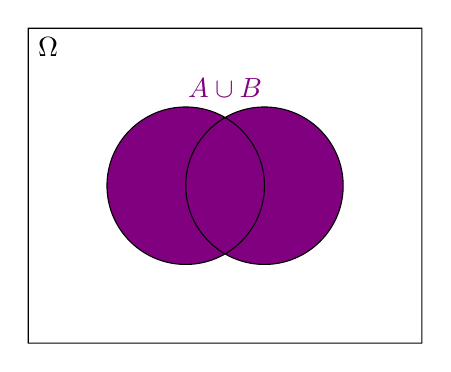
\begin{tikzpicture}[fill=gray, scale=1]
		% left hand
		\scope
		\fill[violet] (0,0) circle (1);
		\endscope
		% right hand
		\scope
		\fill[violet] (1,0) circle (1);
		\endscope
		% outline
		\draw (0,0) circle (1) (0,1) 
		      (1,0) circle (1) (1,1) 
		      (3,-2) rectangle (-2,2) node [text=black,below right] {$\Omega$};
		\draw (.5,1) node [text=black, above, violet] {$A \cup B$};
	\end{tikzpicture}
	\end{center}
			
	Lorsqu'on calcule $P(A) + P(B)$, remarquons qu'on compte deux fois tous les éléments appartenant à la fois à $A$ et à $B$, c'est-à-dire les éléments de $A \cap B$.
	En les retirant une fois, chaque élément de l'union $A\cup B$ est compté une seule fois et on obtient bien
		\[ P(A \cup B) = P(A) + P(B) - P(A\cap B). \]
}{}

\dfn{Événements disjoints}{
	Deux événements $A, B \subseteq \Omega$ sont dits disjoints dès que
		\[ A \cap B = \emptyset, \]
	l'ensemble vide.
	On a dans ce cas et d'après le théorème \ref{thm:incl-excl},
		\[ P(A \cup B) = P(A) + P(B). \]
}{}

\dfn{Équiprobabilité}{
	On parle de situation \emph{équiprobable} si chaque issue $\omega$ de l'univers $\Omega$ admet la même probabilité.
		\[ P(\omega_1) = P(\omega_2) =  P(\omega_3) = \dots, \]
	La loi qui en découle s'appelle la \emph{loi uniforme}.
}{}

\cor{}{
	En situation d'équiprobabilité, chaque issue $\omega$ a pour probabilité
		\[ P(\omega) = \dfrac{1}{\text{Nombre d'issues possibles}} = \dfrac{1}{|\Omega|}. \]
	De plus, chaque événement $E \subseteq \Omega$ a pour probabilité
		\[ P(E) = \dfrac{|E|}{|\Omega|}. \]
}{cor:equiprob}
\pf{Démonstration du corollaire \ref{cor:equiprob}}{
	Comme la probabilité de l'univers $P(\Omega)$ vaut $1$, on en déduit que
		\[ P(\Omega) = P(\omega_1) + P(\omega_2) + \dots  = 1. \]
	Chaque probabilité est la même ; notons la $p$. La somme a exactement $|\Omega|$ termes, donc
		\begin{gather*}
			|\Omega| \cdot p = 1, \\
			p = \dfrac{1}{|\Omega|}. 
		\end{gather*}
	Pour un événement $E = \{e_1, e_2, \dots \} \subseteq \Omega$, on a par définition que la probabilité de l'événement $E$ est la somme de la probabilité de chacun de ses éléments.
		\begin{align*}
			P(E) &= P(e_1) + P(e_2) + \dots \\
				&= \dfrac{1}{|\Omega|} + \dfrac{1}{|\Omega|} + \dots + \dfrac{1}{|\Omega|} \\
				&= \dfrac{|E|}{|\Omega|}.
		\end{align*}
}{}

\dfn{Événement complémentaire}{
	Soit $E \subseteq \Omega$ un événement.
	On pose $\overline{E}$ l'événement complémentaire à $E$ dans $\Omega$ : c'est l'ensemble des issues de $\Omega$ qui n'appartiennent pas à $E$.
	Autrement dit,
		\begin{align*}
			E \cap \overline{E} = \emptyset && \text{et} && E \cup \overline{E} = \Omega.
		\end{align*}
}{}

\nt{
	On note aussi le complémentaire d'un événement $E$ des façons suivantes.
		\[ \overline{E} = E^c = \Omega \setminus E = \Omega - E. \]
}{}

\cor{}{
	Soient $E \subseteq \Omega$ un événement et $\overline{E}$ son complémentaire.
	Alors
		\[ P\left( \overline{E} \right) = 1 - P(E). \]
}{cor:compl}

\pf{Démonstration du corollaire \ref{cor:compl}}{
	En utilisant les propriétés de $P$, du complémentaire, et le principe d'inclusion-exclusion, on trouve
		\begin{align*}
		 1 = P(\Omega) &= P\left( E \cup \overline{E} \right) \\
		 				&= P(E) + P\left(\overline{E}\right) - P\left( E \cap \overline{E}\right) \\
		 				&= P(E) + P\left(\overline{E}\right) - P\left( \emptyset \right) \\
		 				&= P(E) + P\left(\overline{E}\right),
		\end{align*}
	ce qui conclut.
}{}

\section{Arbres de probabilité}

Les arbres de probabilité sont des schémas permettant de décrire les chemins possibles d'une expérience aléatoire à plusieurs épreuves (ou étapes).
Le point de départ est la \emph{racine} de l'arbre, et les issues possibles sont ses \emph{feuilles}.

On choisit ici de représenter un arbre de haut en bas, plutôt que de gauche à droite comme il est commun de le faire.
Il va de soi que ces deux représentations sont identiques.

La \emph{profondeur} de l'arbre désigne le nombre total d'épreuves de l'expérience.
On lit l'arbre en le parcourant de haut en bas, chaque embranchement correspondant à un résultat possible de l'épreuve d'après.
La somme des probabilités de chaque branche est donc nécessairement $1$.
Pour connaître la probabilité d'une issue, il faut multiplier les probabilités correspondant à chaque choix du parcours vers celle-ci.

L'ensemble des feuilles $\omega$ de l'arbre correspond à l'univers $\Omega$ de l'expérience.
On pourra donc connaître $|\Omega|$ en comptant les feuilles, et $P(\omega)$ en multipliant les probabilités qui mènent de la racine à la feuille.

\ex{}{
	On lance un D$6$ équilibré, dé à $6$ faces.
	\begin{enumerate}[label=$\bullet$]
		\item Si le numéro obtenu est un multiple de 3, on extrait au hasard une boule dans l'urne 1 qui contient 3 boules noires, 4 boules blanches et 3 boules rouges
		\item Si le numéro obtenu n'est pas un multiple de 3, on extrait une boule dans l'urne 2 qui contient 3 boules noires et 2 boules blanches.
	\end{enumerate}
	On distingue deux étapes à l'expérience : on crée donc l'arbre de profondeur $2$ suivant, où on dénote par B, N, et R les évéments \og tirer une boule blanche, noire, rouge \fg respectivement.
	
	\begin{center}
	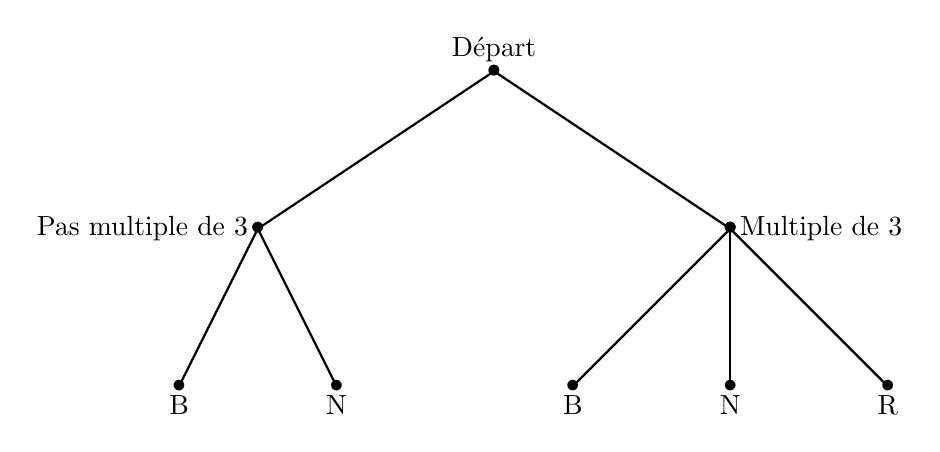
\begin{tikzpicture}
		% depth 1
		\foreach \i in {-3, 3}
		\draw[-, thick, black] (0,0) node {$\bullet$} -- (\i,-2);
		% depth 2
		\foreach \i in {3} \foreach \j in {-2, 0, 2}
			\draw[-, thick, black] (\i,-2) node {$\bullet$} -- (\i+\j,-4) node {$\bullet$};
			
		\foreach \i in {-3} \foreach \j in {-1, 1}
			\draw[-, thick, black] (\i,-2) node {$\bullet$} -- (\i+\j,-4) node {$\bullet$};
			
		\draw (0,0) node[above] {Départ};
		\draw (3,-2) node[right] {Multiple de $3$};
		\draw (-3,-2) node[left] {Pas multiple de $3$};
		\draw (-4,-4) node[below] {B};
		\draw (-2,-4) node[below] {N};
		\draw (1,-4) node[below] {B};
		\draw (3,-4) node[below] {N};
		\draw (5,-4) node[below] {R};
	\end{tikzpicture}
	\end{center}
	On ajoute les probabilités de chacun des événements sur les branches associées.
	Par exemple, de la racine, pour atteindre l'embranchement \og multiple de $3$ \fg, il y a $1$ chance sur $3$ (car seuls $3$ et $6$ sont les issues favorables).
	On ajoute donc un $\frac13$ sur la brache qui mène à cet événement, est un $\frac23$ sur l'autre.
	
	En sachant qu'on ait obtenu un nombre qui n'est pas un multiple de $3$, on tire une boule dans la deuxième urne  qui contient 3 boules noires et 2 boules blanches.
	La probabilité d'obtenir une boule blanche est donc $\frac25$, et celle d'obtenir une boule noire est $\frac35$.
	En notant toutes les probabilités ainsi calculées, on obtient l'arbre de probabilité suivant.
	
	\begin{center}
	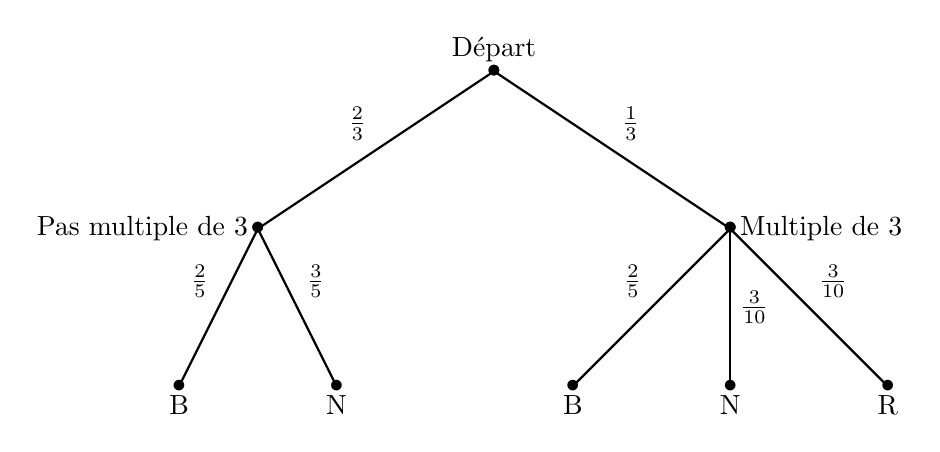
\begin{tikzpicture}
		% depth 1
		\foreach \i in {-3, 3}
		\draw[-, thick, black] (0,0) node {$\bullet$} -- (\i,-2);
		% depth 2
		\foreach \i in {3} \foreach \j in {-2, 0, 2}
			\draw[-, thick, black] (\i,-2) node {$\bullet$} -- (\i+\j,-4) node {$\bullet$};
			
		\foreach \i in {-3} \foreach \j in {-1, 1}
			\draw[-, thick, black] (\i,-2) node {$\bullet$} -- (\i+\j,-4) node {$\bullet$};
			
		\draw (0,0) node[above] {Départ};
		\draw (3,-2) node[right] {Multiple de $3$};
		\draw (-3,-2) node[left] {Pas multiple de $3$};
		\draw (-4,-4) node[below] {B};
		\draw (-2,-4) node[below] {N};
		\draw (1,-4) node[below] {B};
		\draw (3,-4) node[below] {N};
		\draw (5,-4) node[below] {R};
		
		\draw (-1.5, -1) node[above left] {$\frac23$};
		\draw (1.5, -1) node[above right] {$\frac13$};
		
		\draw (-3.5, -3) node[above left] {$\frac25$};
		\draw (-2.5, -3) node[above right] {$\frac35$};
		
		\draw (2, -3) node[above left] {$\frac25$};
		\draw (3, -3) node[right] {$\frac3{10}$};
		\draw (4, -3) node[above right] {$\frac3{10}$};
	\end{tikzpicture}
	\end{center}
	On calcule par exemple
		\[ P(N) = \dfrac23 \cdot \dfrac35 + \dfrac13 \cdot \dfrac3{10} = \dfrac12. \]
}{}


\section{Construction d'un modèle empirique}

Lorsqu'on étudie une expérience aléatoire, il n'est pas toujours simple de connaître \emph{a priori} la probabilité de chacune des issues possibles.
Par exemple, même si un dé à $6$ faces est su pipé, il n'est pas possible de connaître la probabilité d'obtenir un $6$ : elle pourrait être $1$ (si la face $6$ est lestée), comme $0$ (si une autre face l'est), comme toute autre valeur entre $0$ et $1$.

Une façon naturelle de connaître la probabilité d'obtenir un $6$ est donc de lancer le dé un grand nombre de fois.
La fréquence d'apparition de $6$ parmis toutes les autres issues donnera donc une \emph{approximation} de la probabilité recherchée, qu'on \emph{admettra} ensuite comme probabilité dans notre modèle afin de prédire le résultat des lancers suivants.

Cette construction de modèle probabiliste est empirique : elle ne s'appuie que sur l'expérience et sur l'hypothèse que le lancer de dé est une expérience aléatoire bien définie (les probabilités ne changent pas d'un lancer à l'autre).
L'erreur commise entre une probabilité réelle et une fréquence dépend du nombre d'expériences réalisées.
L'inégalité de Chebyshev permet de montrer formellement qu'une telle fréquence est proche de sa moyenne lorsque sa variance diminue.
Cela rejoint l'interprétation de l'écart type donnée dans le chapitre \ref{chap:stats}.

